\documentclass{standalone}
\usepackage{tikz}
\usetikzlibrary{patterns, positioning}
\usepackage[sfdefault]{ClearSans} %% option 'sfdefault' activates Clear Sans as the default text font
\usepackage[T1]{fontenc}

\begin{document}
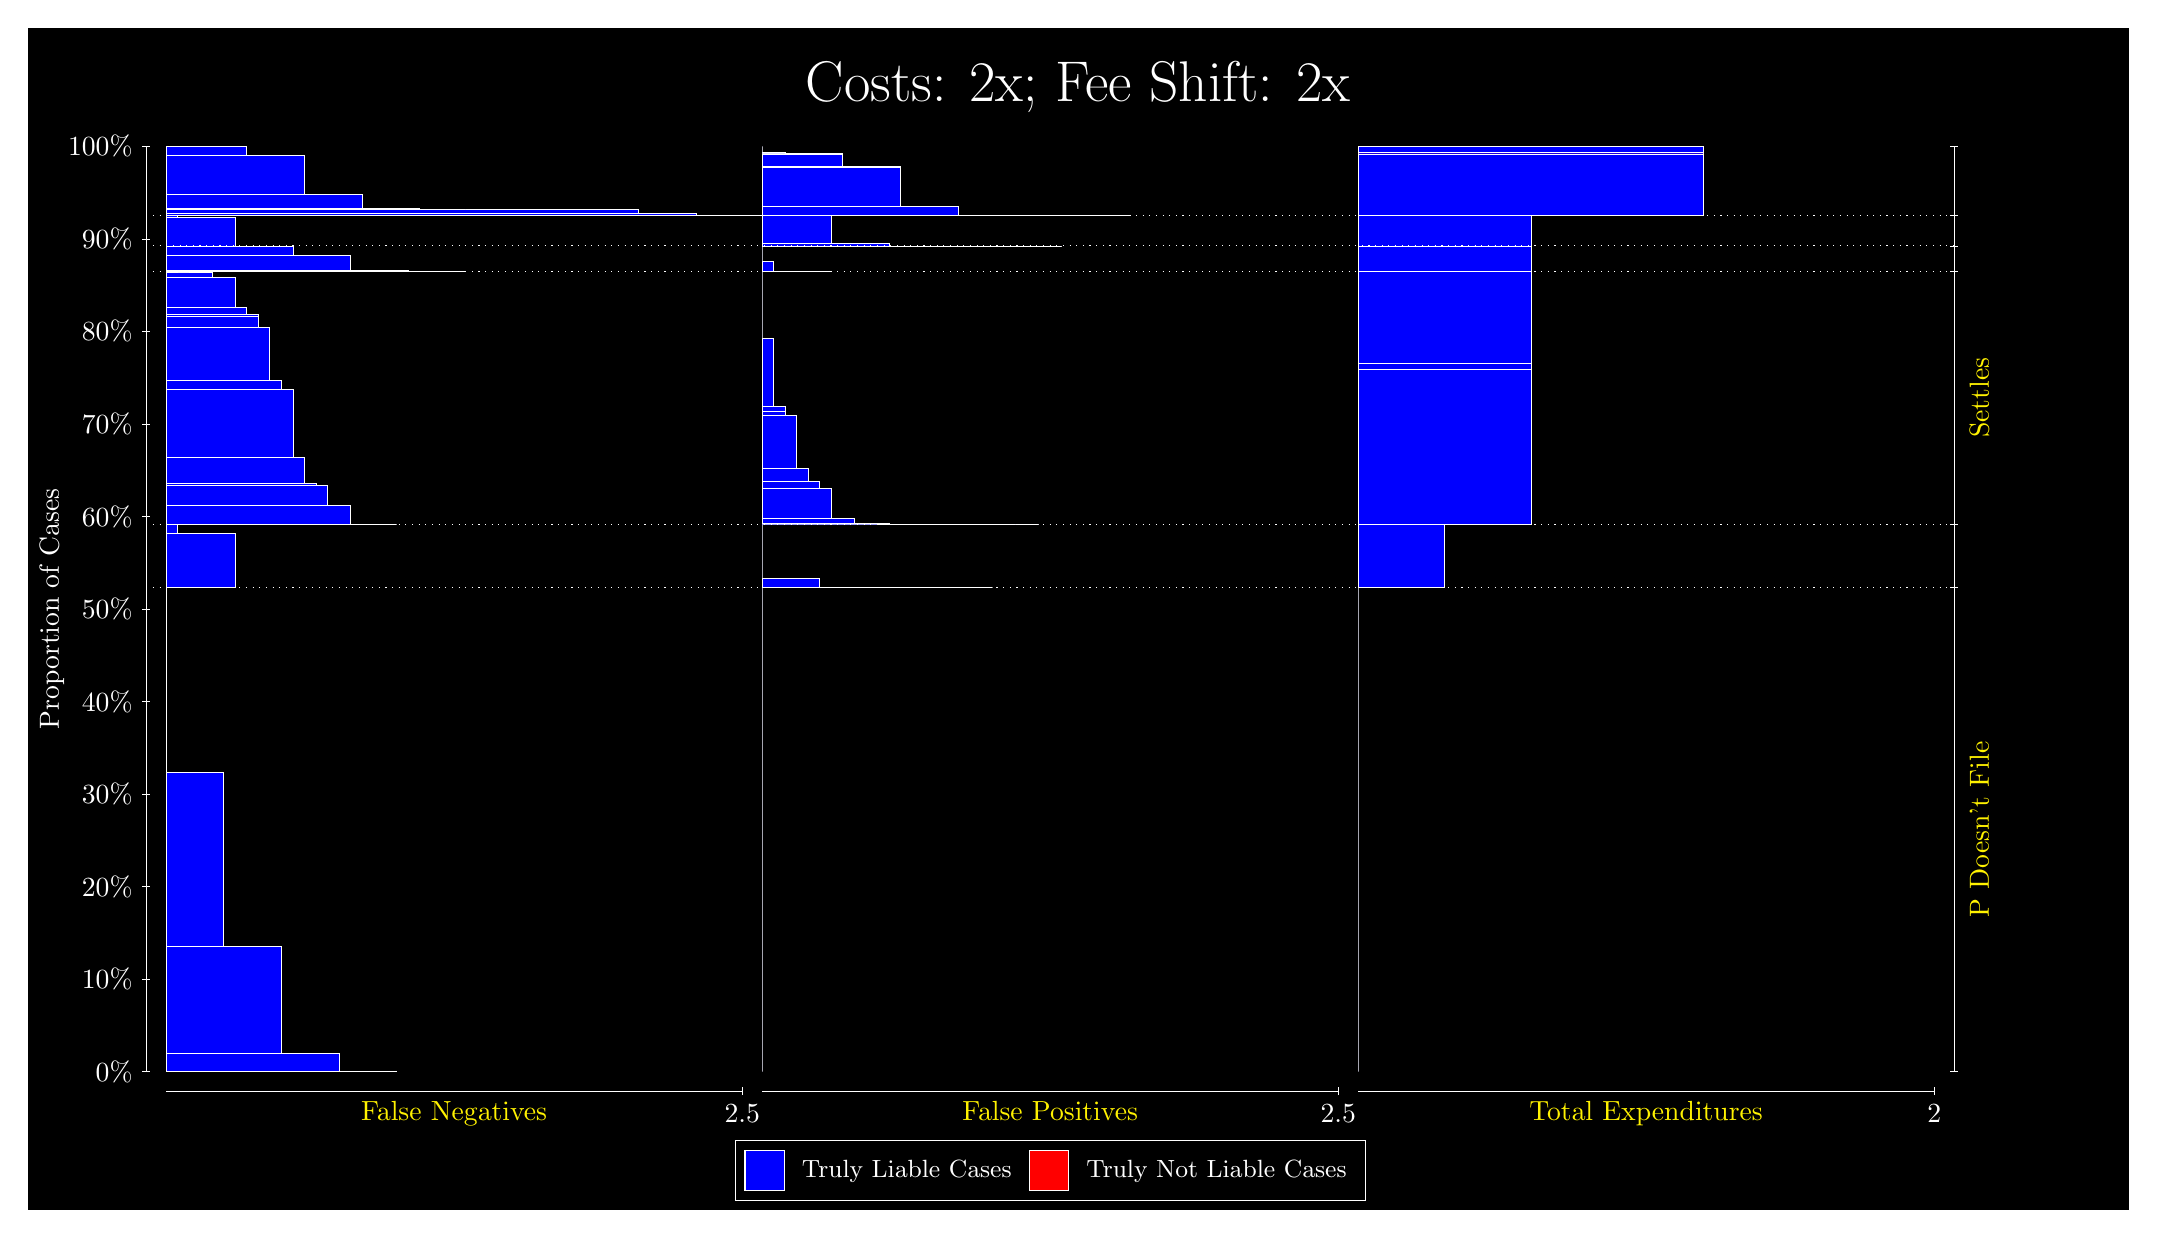
\begin{tikzpicture}
\draw[fill=black] (0,0) rectangle (26.667,15);
\draw[text=white] (0,13.5) rectangle (26.667,15) node[midway] {\huge Costs: 2x; Fee Shift: 2x};
\draw[white, very thin] (1.5,1.75) -- (1.5,13.5);
\node[rotate=90, text=white, anchor=center] at (0.3, 7.625) {Proportion of Cases};
\draw[white, very thin] (1.45,1.75) -- (1.55,1.75);
\node[text=white, anchor=east] at (1.45, 1.75) {0\%};
\draw[white, very thin] (1.45,2.925) -- (1.55,2.925);
\node[text=white, anchor=east] at (1.45, 2.925) {10\%};
\draw[white, very thin] (1.45,4.1) -- (1.55,4.1);
\node[text=white, anchor=east] at (1.45, 4.1) {20\%};
\draw[white, very thin] (1.45,5.275) -- (1.55,5.275);
\node[text=white, anchor=east] at (1.45, 5.275) {30\%};
\draw[white, very thin] (1.45,6.45) -- (1.55,6.45);
\node[text=white, anchor=east] at (1.45, 6.45) {40\%};
\draw[white, very thin] (1.45,7.625) -- (1.55,7.625);
\node[text=white, anchor=east] at (1.45, 7.625) {50\%};
\draw[white, very thin] (1.45,8.8) -- (1.55,8.8);
\node[text=white, anchor=east] at (1.45, 8.8) {60\%};
\draw[white, very thin] (1.45,9.975) -- (1.55,9.975);
\node[text=white, anchor=east] at (1.45, 9.975) {70\%};
\draw[white, very thin] (1.45,11.15) -- (1.55,11.15);
\node[text=white, anchor=east] at (1.45, 11.15) {80\%};
\draw[white, very thin] (1.45,12.325) -- (1.55,12.325);
\node[text=white, anchor=east] at (1.45, 12.325) {90\%};
\draw[white, very thin] (1.45,13.5) -- (1.55,13.5);
\node[text=white, anchor=east] at (1.45, 13.5) {100\%};

\draw[white, very thin] (24.457,1.75) -- (24.457,13.5);
\draw[white, very thin] (24.407,1.75) -- (24.507,1.75);
\node[anchor=west] at (24.407, 1.75) {};
\draw[white, very thin] (24.407,7.8972) -- (24.507,7.8972);
\node[anchor=west] at (24.407, 7.8972) {};
\draw[white, very thin] (24.407,8.7004) -- (24.507,8.7004);
\node[anchor=west] at (24.407, 8.7004) {};
\draw[white, very thin] (24.407,11.913) -- (24.507,11.913);
\node[anchor=west] at (24.407, 11.913) {};
\draw[white, very thin] (24.407,12.235) -- (24.507,12.235);
\node[anchor=west] at (24.407, 12.235) {};
\draw[white, very thin] (24.407,12.626) -- (24.507,12.626);
\node[anchor=west] at (24.407, 12.626) {};
\draw[white, very thin] (24.407,13.5) -- (24.507,13.5);
\node[anchor=west] at (24.407, 13.5) {};

\draw[white, very thin, fill=blue] (1.75,1.75) rectangle (4.6775,1.7523);
\draw[white, very thin, fill=blue] (1.75,1.7523) rectangle (3.9457,1.9834);
\draw[white, very thin, fill=blue] (1.75,1.9834) rectangle (3.2138,3.3441);
\draw[white, very thin, fill=blue] (1.75,3.3441) rectangle (2.4819,5.5487);
\draw[white, very thin, fill=red] (1.75,5.5487) rectangle (1.75,5.5487);
\draw[white, very thin, fill=blue] (1.75,5.5487) rectangle (1.75,7.8972);
\draw[white, very thin, fill=blue] (1.75,7.8972) rectangle (2.6283,8.5802);
\draw[white, very thin, fill=blue] (1.75,8.5802) rectangle (1.8964,8.6999);
\draw[white, very thin, fill=red] (1.75,8.6999) rectangle (1.75,8.6999);
\draw[white, very thin, fill=blue] (1.75,8.6999) rectangle (1.75,8.7004);
\draw[white, very thin, fill=blue] (1.75,8.7004) rectangle (4.6775,8.7004);
\draw[white, very thin, fill=blue] (1.75,8.7004) rectangle (4.3848,8.7006);
\draw[white, very thin, fill=blue] (1.75,8.7006) rectangle (4.092,8.9421);
\draw[white, very thin, fill=blue] (1.75,8.9421) rectangle (3.9457,8.9463);
\draw[white, very thin, fill=blue] (1.75,8.9463) rectangle (3.7993,9.1939);
\draw[white, very thin, fill=blue] (1.75,9.1939) rectangle (3.6529,9.2237);
\draw[white, very thin, fill=blue] (1.75,9.2237) rectangle (3.5065,9.5506);
\draw[white, very thin, fill=blue] (1.75,9.5506) rectangle (3.3602,10.415);
\draw[white, very thin, fill=blue] (1.75,10.415) rectangle (3.2138,10.532);
\draw[white, very thin, fill=blue] (1.75,10.532) rectangle (3.0674,11.202);
\draw[white, very thin, fill=blue] (1.75,11.202) rectangle (2.921,11.34);
\draw[white, very thin, fill=blue] (1.75,11.34) rectangle (2.921,11.362);
\draw[white, very thin, fill=blue] (1.75,11.362) rectangle (2.7746,11.453);
\draw[white, very thin, fill=blue] (1.75,11.453) rectangle (2.6283,11.835);
\draw[white, very thin, fill=blue] (1.75,11.835) rectangle (2.4819,11.841);
\draw[white, very thin, fill=blue] (1.75,11.841) rectangle (2.3355,11.897);
\draw[white, very thin, fill=blue] (1.75,11.897) rectangle (2.1891,11.903);
\draw[white, very thin, fill=blue] (1.75,11.903) rectangle (2.1891,11.904);
\draw[white, very thin, fill=blue] (1.75,11.904) rectangle (2.0428,11.904);
\draw[white, very thin, fill=blue] (1.75,11.904) rectangle (1.8964,11.913);
\draw[white, very thin, fill=red] (1.75,11.913) rectangle (1.75,11.913);
\draw[white, very thin, fill=blue] (1.75,11.913) rectangle (1.75,11.913);
\draw[white, very thin, fill=blue] (1.75,11.913) rectangle (5.5558,11.913);
\draw[white, very thin, fill=blue] (1.75,11.913) rectangle (4.8239,11.92);
\draw[white, very thin, fill=blue] (1.75,11.92) rectangle (4.092,12.11);
\draw[white, very thin, fill=blue] (1.75,12.11) rectangle (3.3602,12.234);
\draw[white, very thin, fill=blue] (1.75,12.234) rectangle (2.6283,12.235);
\draw[white, very thin, fill=red] (1.75,12.235) rectangle (1.75,12.235);
\draw[white, very thin, fill=blue] (1.75,12.235) rectangle (2.6283,12.595);
\draw[white, very thin, fill=blue] (1.75,12.595) rectangle (1.8964,12.626);
\draw[white, very thin, fill=red] (1.75,12.626) rectangle (1.75,12.626);
\draw[white, very thin, fill=blue] (1.75,12.626) rectangle (1.75,12.626);
\draw[white, very thin, fill=blue] (1.75,12.626) rectangle (9.9471,12.626);
\draw[white, very thin, fill=blue] (1.75,12.626) rectangle (9.2152,12.627);
\draw[white, very thin, fill=blue] (1.75,12.627) rectangle (8.4834,12.645);
\draw[white, very thin, fill=blue] (1.75,12.645) rectangle (7.7515,12.704);
\draw[white, very thin, fill=blue] (1.75,12.704) rectangle (7.0196,12.705);
\draw[white, very thin, fill=blue] (1.75,12.705) rectangle (6.2877,12.705);
\draw[white, very thin, fill=blue] (1.75,12.705) rectangle (5.7022,12.705);
\draw[white, very thin, fill=blue] (1.75,12.705) rectangle (5.5558,12.705);
\draw[white, very thin, fill=blue] (1.75,12.705) rectangle (4.9703,12.709);
\draw[white, very thin, fill=blue] (1.75,12.709) rectangle (4.2384,12.885);
\draw[white, very thin, fill=blue] (1.75,12.885) rectangle (3.5065,13.39);
\draw[white, very thin, fill=blue] (1.75,13.39) rectangle (2.7746,13.496);
\draw[white, very thin, fill=blue] (1.75,13.496) rectangle (2.0428,13.5);
\draw[white, very thin, fill=red] (1.75,13.5) rectangle (1.75,13.5);
\draw[white, very thin, fill=blue] (1.75,13.5) rectangle (1.75,13.5);
\draw[white, very thin, fill=red] (9.3189,1.75) rectangle (9.3189,1.75);
\draw[white, very thin, fill=blue] (9.3189,1.75) rectangle (9.3189,7.8972);
\draw[white, very thin, fill=red] (9.3189,7.8972) rectangle (12.246,7.8972);
\draw[white, very thin, fill=blue] (9.3189,7.8972) rectangle (12.246,7.8972);
\draw[white, very thin, fill=blue] (9.3189,7.8972) rectangle (11.515,7.8972);
\draw[white, very thin, fill=blue] (9.3189,7.8972) rectangle (10.783,7.8977);
\draw[white, very thin, fill=blue] (9.3189,7.8977) rectangle (10.051,8.0174);
\draw[white, very thin, fill=blue] (9.3189,8.0174) rectangle (9.3189,8.7004);
\draw[white, very thin, fill=red] (9.3189,8.7004) rectangle (12.832,8.7004);
\draw[white, very thin, fill=blue] (9.3189,8.7004) rectangle (12.832,8.7004);
\draw[white, very thin, fill=red] (9.3189,8.7004) rectangle (12.539,8.7004);
\draw[white, very thin, fill=blue] (9.3189,8.7004) rectangle (12.539,8.7004);
\draw[white, very thin, fill=red] (9.3189,8.7004) rectangle (12.246,8.7004);
\draw[white, very thin, fill=blue] (9.3189,8.7004) rectangle (12.246,8.7004);
\draw[white, very thin, fill=blue] (9.3189,8.7004) rectangle (12.1,8.7004);
\draw[white, very thin, fill=red] (9.3189,8.7004) rectangle (11.954,8.7004);
\draw[white, very thin, fill=blue] (9.3189,8.7004) rectangle (11.954,8.7004);
\draw[white, very thin, fill=blue] (9.3189,8.7004) rectangle (11.807,8.7004);
\draw[white, very thin, fill=red] (9.3189,8.7004) rectangle (11.661,8.7004);
\draw[white, very thin, fill=blue] (9.3189,8.7004) rectangle (11.661,8.7004);
\draw[white, very thin, fill=blue] (9.3189,8.7004) rectangle (11.515,8.7004);
\draw[white, very thin, fill=red] (9.3189,8.7004) rectangle (11.368,8.7004);
\draw[white, very thin, fill=blue] (9.3189,8.7004) rectangle (11.368,8.7004);
\draw[white, very thin, fill=blue] (9.3189,8.7004) rectangle (11.222,8.7004);
\draw[white, very thin, fill=blue] (9.3189,8.7004) rectangle (11.075,8.7004);
\draw[white, very thin, fill=red] (9.3189,8.7004) rectangle (11.075,8.7004);
\draw[white, very thin, fill=blue] (9.3189,8.7004) rectangle (11.075,8.7004);
\draw[white, very thin, fill=blue] (9.3189,8.7004) rectangle (10.929,8.7086);
\draw[white, very thin, fill=blue] (9.3189,8.7086) rectangle (10.783,8.7088);
\draw[white, very thin, fill=blue] (9.3189,8.7088) rectangle (10.636,8.7159);
\draw[white, very thin, fill=blue] (9.3189,8.7159) rectangle (10.49,8.7723);
\draw[white, very thin, fill=blue] (9.3189,8.7723) rectangle (10.344,8.7742);
\draw[white, very thin, fill=blue] (9.3189,8.7742) rectangle (10.344,8.7779);
\draw[white, very thin, fill=blue] (9.3189,8.7779) rectangle (10.197,9.1599);
\draw[white, very thin, fill=blue] (9.3189,9.1599) rectangle (10.051,9.2514);
\draw[white, very thin, fill=blue] (9.3189,9.2514) rectangle (9.9044,9.4109);
\draw[white, very thin, fill=blue] (9.3189,9.4109) rectangle (9.758,10.081);
\draw[white, very thin, fill=blue] (9.3189,10.081) rectangle (9.6116,10.131);
\draw[white, very thin, fill=blue] (9.3189,10.131) rectangle (9.6116,10.198);
\draw[white, very thin, fill=blue] (9.3189,10.198) rectangle (9.4652,11.062);
\draw[white, very thin, fill=blue] (9.3189,11.062) rectangle (9.3189,11.913);
\draw[white, very thin, fill=red] (9.3189,11.913) rectangle (10.197,11.913);
\draw[white, very thin, fill=blue] (9.3189,11.913) rectangle (10.197,11.914);
\draw[white, very thin, fill=blue] (9.3189,11.914) rectangle (9.4652,12.038);
\draw[white, very thin, fill=blue] (9.3189,12.038) rectangle (9.3189,12.235);
\draw[white, very thin, fill=red] (9.3189,12.235) rectangle (13.125,12.235);
\draw[white, very thin, fill=blue] (9.3189,12.235) rectangle (13.125,12.235);
\draw[white, very thin, fill=blue] (9.3189,12.235) rectangle (12.393,12.235);
\draw[white, very thin, fill=blue] (9.3189,12.235) rectangle (11.661,12.236);
\draw[white, very thin, fill=blue] (9.3189,12.236) rectangle (10.929,12.266);
\draw[white, very thin, fill=blue] (9.3189,12.266) rectangle (10.197,12.626);
\draw[white, very thin, fill=red] (9.3189,12.626) rectangle (14.003,12.626);
\draw[white, very thin, fill=blue] (9.3189,12.626) rectangle (14.003,12.626);
\draw[white, very thin, fill=red] (9.3189,12.626) rectangle (13.271,12.626);
\draw[white, very thin, fill=blue] (9.3189,12.626) rectangle (13.271,12.626);
\draw[white, very thin, fill=red] (9.3189,12.626) rectangle (12.539,12.626);
\draw[white, very thin, fill=blue] (9.3189,12.626) rectangle (12.539,12.63);
\draw[white, very thin, fill=blue] (9.3189,12.63) rectangle (11.807,12.736);
\draw[white, very thin, fill=red] (9.3189,12.736) rectangle (11.807,12.736);
\draw[white, very thin, fill=blue] (9.3189,12.736) rectangle (11.807,12.736);
\draw[white, very thin, fill=blue] (9.3189,12.736) rectangle (11.075,13.24);
\draw[white, very thin, fill=blue] (9.3189,13.24) rectangle (11.075,13.241);
\draw[white, very thin, fill=blue] (9.3189,13.241) rectangle (10.344,13.402);
\draw[white, very thin, fill=blue] (9.3189,13.402) rectangle (10.344,13.417);
\draw[white, very thin, fill=blue] (9.3189,13.417) rectangle (9.6116,13.421);
\draw[white, very thin, fill=blue] (9.3189,13.421) rectangle (9.6116,13.421);
\draw[white, very thin, fill=red] (9.3189,13.421) rectangle (9.3189,13.421);
\draw[white, very thin, fill=blue] (9.3189,13.421) rectangle (9.3189,13.5);
\draw[white, very thin, fill=red] (16.888,1.75) rectangle (16.888,1.75);
\draw[white, very thin, fill=blue] (16.888,1.75) rectangle (16.888,7.8972);
\draw[white, very thin, fill=red] (16.888,7.8972) rectangle (17.986,7.8972);
\draw[white, very thin, fill=blue] (16.888,7.8972) rectangle (17.986,8.7004);
\draw[white, very thin, fill=red] (16.888,8.7004) rectangle (19.083,8.7004);
\draw[white, very thin, fill=blue] (16.888,8.7004) rectangle (19.083,10.667);
\draw[white, very thin, fill=red] (16.888,10.667) rectangle (19.083,10.667);
\draw[white, very thin, fill=blue] (16.888,10.667) rectangle (19.083,10.742);
\draw[white, very thin, fill=red] (16.888,10.742) rectangle (19.083,10.742);
\draw[white, very thin, fill=blue] (16.888,10.742) rectangle (19.083,11.913);
\draw[white, very thin, fill=red] (16.888,11.913) rectangle (19.083,11.913);
\draw[white, very thin, fill=blue] (16.888,11.913) rectangle (19.083,12.235);
\draw[white, very thin, fill=red] (16.888,12.235) rectangle (19.083,12.235);
\draw[white, very thin, fill=blue] (16.888,12.235) rectangle (19.083,12.626);
\draw[white, very thin, fill=red] (16.888,12.626) rectangle (21.279,12.626);
\draw[white, very thin, fill=blue] (16.888,12.626) rectangle (21.279,13.405);
\draw[white, very thin, fill=red] (16.888,13.405) rectangle (21.279,13.405);
\draw[white, very thin, fill=blue] (16.888,13.405) rectangle (21.279,13.421);
\draw[white, very thin, fill=red] (16.888,13.421) rectangle (21.279,13.421);
\draw[white, very thin, fill=blue] (16.888,13.421) rectangle (21.279,13.5);
\draw[white, dotted] (1.5,7.8972) -- (24.457,7.8972);
\draw[white, dotted] (1.5,8.7004) -- (24.457,8.7004);
\draw[white, dotted] (1.5,11.913) -- (24.457,11.913);
\draw[white, dotted] (1.5,12.235) -- (24.457,12.235);
\draw[white, dotted] (1.5,12.626) -- (24.457,12.626);
\draw[white, very thin] (1.75,1.5) -- (9.0689,1.5);
\node[text=yellow, anchor=north] at (5.4094, 1.5) {False Negatives};
\draw[white, very thin] (9.0689,1.45) -- (9.0689,1.55);
\node[text=white, anchor=north] at (9.0689, 1.45) {2.5};

\draw[white, very thin] (9.3189,1.5) -- (16.638,1.5);
\node[text=yellow, anchor=north] at (12.978, 1.5) {False Positives};
\draw[white, very thin] (16.638,1.45) -- (16.638,1.55);
\node[text=white, anchor=north] at (16.638, 1.45) {2.5};

\draw[white, very thin] (16.888,1.5) -- (24.207,1.5);
\node[text=yellow, anchor=north] at (20.547, 1.5) {Total Expenditures};
\draw[white, very thin] (24.207,1.45) -- (24.207,1.55);
\node[text=white, anchor=north] at (24.207, 1.45) {2};

\node[text=yellow, centered, rotate=90] at (24.777, 4.8236) {P Doesn't File};

\node[text=yellow, centered, rotate=90] at (24.777, 10.307) {Settles};




\draw (12.978300999999998,1.5) node[draw=none] (baseCoordinate) {};
\begin{scope}[align=center]
        \matrix[scale=0.5, draw=white, below=0.5cm of baseCoordinate, nodes={draw}, column sep=0.1cm]{
            \node[rectangle, draw, minimum width=0.5cm, minimum height=0.5cm, fill=blue] {}; &
            \node[draw=none, font=\small, text=white] (B) {Truly Liable Cases}; &
            \node[rectangle, draw, minimum width=0.5cm, minimum height=0.5cm, fill=red] {}; &
            \node[draw=none, font=\small, text=white] (B) {Truly Not Liable Cases}; \\
            };
\end{scope}

\end{tikzpicture}
\end{document}